%%%%%%%%%%%%%%%%%%%%%%%%%%%%%%%%%%%%%%%%%%%%%%%%%%%%%%%%%%%%%%%%%%%%%%%% 
%%%%%%%%%%%%%%%%%%%%%%%%%%%%%%%%%%%%%%%%%%%%%%%%%%%%%%%%%%%%%%%%%%%%%%%% 
\begin{frame}
  \frametitle{The future of portable asynchonous tasking}

  {\large \textcolor{darkgreen}{{\bf HiHAT initiative:} Hierarchical Heterogenous Asynchronous Tasking}}

  \begin{itemize}
  \item for Runtime frameworks developpers + HW vendors
  \item<1> Tasking frameworks
  \item<2> Fonctionalities
  \end{itemize}
  
  \only<1>{
    \begin{center}
      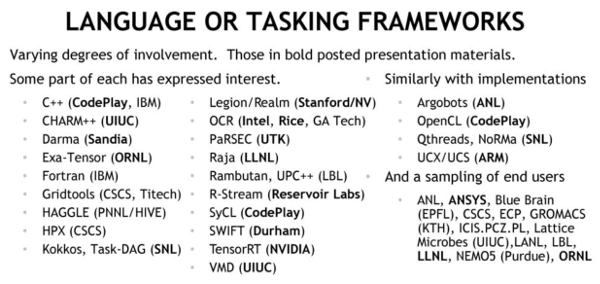
\includegraphics[height=5.0cm]{doc/perf_portability/hihat/hihat_1b}
    \end{center}
  }
  \only<2>{
    \begin{center}
      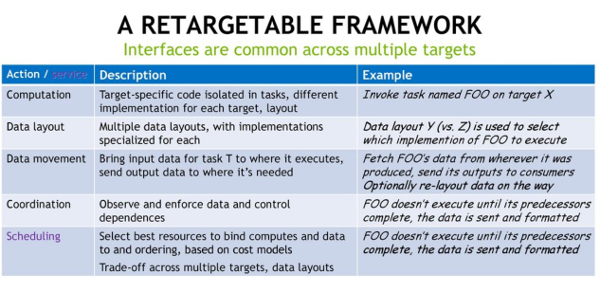
\includegraphics[height=5.0cm]{doc/perf_portability/hihat/hihat_2b}
    \end{center}
  }

  {\small
    reference \myhref{https://wiki.modelado.org/images/5/54/HiHAT_Mini-Summit_17_Overview.pdf}{HiHAT\_Mini-Summit\_17\_Overview.pdf}\\
    reference \myurl{http://slideplayer.com/slide/12990108/}
  }

\end{frame}

%%%%%%%%%%%%%%%%%%%%%%%%%%%%%%%%%%%%%%%%%%%%%%%%%%%%%%%%%%%%%%%%%%%%%%%% 
%%%%%%%%%%%%%%%%%%%%%%%%%%%%%%%%%%%%%%%%%%%%%%%%%%%%%%%%%%%%%%%%%%%%%%%% 
\begin{frame}
  \frametitle{AMT : Asynchonous Many Task frameworks}
  
  \begin{itemize}
  \item \myhref{https://github.com/StanfordLegion/legion}{Legion} (Stanford)
  \item \myhref{http://starpu.gforge.inria.fr/}{StarPU} (Inria Bordeaux)
  \item \myhref{https://share-ng.sandia.gov/darma/}{DARMA} (Sandia NL)
  \item \myhref{http://charmplusplus.org/}{Charm++} (Univ. Illinois, Urban Champain)
  \item \myhref{http://uintah.sci.utah.edu/}{Uintah}
  \end{itemize}

  \myhref{https://share-ng.sandia.gov/darma/_assets/documents/Sandia2015_AMT_RTS_L2.pdf}{Comparative analysis of Legion, Charm++, Uintah}

\end{frame}
